%========================================
% LESSON CONTENT: Ecuaciones
%========================================

\lesson{Ecuaciones}

%========================================
% SECTION 3.1: Definición y Terminología
%========================================
\subsectiontitle{Ecuaciones: Definición y Terminología}

\begin{definition}
Una \textbf{ecuación} es un enunciado de igualdad entre dos expresiones algebraicas.
\end{definition}

\begin{example}
Ejemplos de ecuaciones:
\begin{align}
8x^3 + x - 9 &= 6x - 1\\
3x + 8 &= 6\\
\frac{3x}{5x+1} &= 9\\
(1+x)^2 &= 5x^2 - 7
\end{align}
\end{example}

\begin{definition}
Una \textbf{solución} de una ecuación es el valor o valores que hacen cierta la ecuación; decimos que estos valores "satisfacen" la ecuación.
\end{definition}

% Visual representation of equation verification
\begin{center}
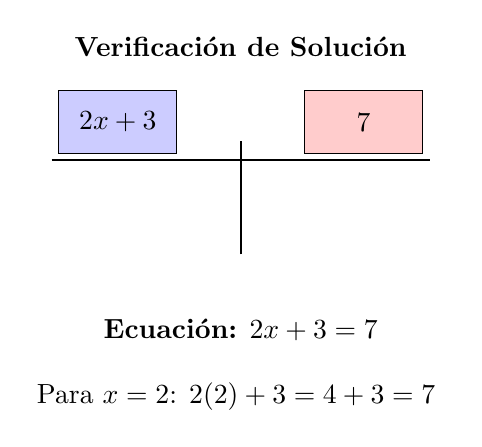
\begin{tikzpicture}[scale=1.2]
    % Balance scale
    \draw[thick] (0,0) -- (4,0);
    \draw[thick] (2,-0.2) -- (2,0.2);
    \draw[thick] (2,-1) -- (2,0);
    
    % Left side
    \node[draw, fill=blue!20, minimum width=1.5cm, minimum height=0.8cm] at (0.7,0.4) {$2x + 3$};
    
    % Right side  
    \node[draw, fill=red!20, minimum width=1.5cm, minimum height=0.8cm] at (3.3,0.4) {$7$};
    
    % Equation
    \node at (2,-1.8) {\textbf{Ecuación:} $2x + 3 = 7$};
    
    % Solution verification
    \node at (2,-2.5) {Para $x = 2$: $2(2) + 3 = 4 + 3 = 7$ $\checkmark$};
    
    % Title
    \node at (2,1.2) {\textbf{Verificación de Solución}};
\end{tikzpicture}
\end{center}

\begin{example}
\textbf{Verificación:} Para la ecuación $2x + 3 = 7$, verificamos que $x = 2$ es solución:
$$2(2) + 3 = 4 + 3 = 7 \quad \checkmark$$
\end{example}

\textbf{Terminología por variables:}
\begin{itemize}
\item \textbf{Ecuación en una variable:} involucra una sola variable (ej: $3x + 5 = 11$)
\item \textbf{Ecuación en dos variables:} involucra dos variables (ej: $2x + 3y = 6$)
\item \textbf{Ecuación en $n$ variables:} involucra $n$ variables
\end{itemize}

\begin{definition}
Una \textbf{identidad} es una ecuación que siempre es cierta para todos los valores reales en los dominios de sus expresiones.
\end{definition}

\begin{example}
Ejemplos de identidades:
\begin{align}
-11 &= -11\\
3x &= 3x\\
-x^2 + 4x - 5 &= -x^2 + 4x - 5
\end{align}
\end{example}

%========================================
% SECTION 3.2: Ecuaciones lineales en una variable
%========================================
\subsectiontitle{Ecuaciones lineales en una variable}

\begin{definition}
Una \textbf{ecuación lineal en una variable} es una ecuación que puede escribirse en la forma $ax + b = 0$ donde $a \neq 0$ y $a, b \in \mathbb{R}$.
\end{definition}

\begin{definition}
Dos ecuaciones son \textbf{equivalentes} si tienen las mismas soluciones.
\end{definition}

\begin{example}
Las ecuaciones $2x + 3 = 5$ y $6x + 9 = 15$ son equivalentes porque ambas tienen como solución $x = 1$.
\end{example}

\textbf{Operaciones que producen ecuaciones equivalentes:}
\begin{enumerate}
\item Sumar o restar la misma cantidad a ambos lados
\item Multiplicar o dividir por una misma cantidad distinta de cero
\item Intercambiar los lados sin alterar signos
\end{enumerate}

% Visual flowchart for solving linear equations
\begin{center}
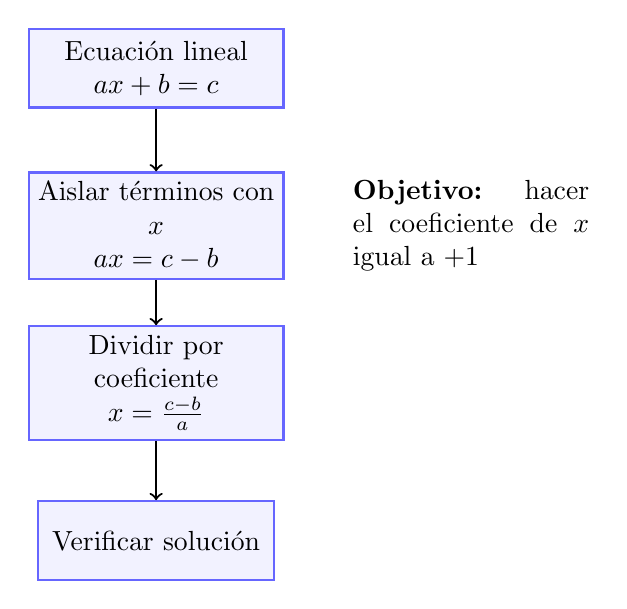
\begin{tikzpicture}[
    stepstyle/.style={rectangle, draw=blue!60, fill=blue!5, thick, minimum width=3cm, text centered, minimum height=1cm},
    arrowstyle/.style={->, thick}
]
    \node[stepstyle] (start) at (0,0) {\parbox{3cm}{\centering Ecuación lineal \\ $ax + b = c$}};
    \node[stepstyle] (isolate) at (0,-2) {\parbox{3cm}{\centering Aislar términos con $x$ \\ $ax = c - b$}};
    \node[stepstyle] (divide) at (0,-4) {\parbox{3cm}{\centering Dividir por coeficiente \\ $x = \frac{c-b}{a}$}};
    \node[stepstyle] (verify) at (0,-6) {Verificar solución};
    
    \draw[arrowstyle] (start) -- (isolate);
    \draw[arrowstyle] (isolate) -- (divide);
    \draw[arrowstyle] (divide) -- (verify);
    
    \node at (4,-2) {\parbox{3cm}{\textbf{Objetivo:} hacer el coeficiente de $x$ igual a $+1$}};
\end{tikzpicture}
\end{center}

\textbf{Procedimiento típico para resolver ecuaciones lineales:}
\begin{enumerate}
\item Evaluar exponentes; eliminar paréntesis y/o fracciones
\item Reunir términos con $x$ a un lado y constantes al otro
\item Dividir por el coeficiente de $x$
\end{enumerate}

\begin{example}
\textbf{Ejemplo 1:} Resolver $3x - 9 = 0$.

\textbf{Solución:}
\begin{align}
3x - 9 &= 0\\
3x &= 9 \quad \text{(sumar 9 a ambos lados)}\\
x &= 3 \quad \text{(dividir entre 3)}
\end{align}

\textbf{Verificación:} $3(3) - 9 = 9 - 9 = 0$ $\checkmark$
\end{example}

\begin{example}
\textbf{Ejemplo 2 (con fracciones):} Resolver $\dfrac{x-1}{5} = \dfrac{2x-1}{7}$.

\textbf{Solución:}
\begin{align}
\frac{x-1}{5} &= \frac{2x-1}{7}\\
35 \cdot \frac{x-1}{5} &= 35 \cdot \frac{2x-1}{7} \quad \text{(multiplicar por MCD = 35)}\\
7(x-1) &= 5(2x-1) \quad \text{(simplificar)}\\
7x - 7 &= 10x - 5 \quad \text{(expandir)}\\
-7 + 5 &= 10x - 7x \quad \text{(reorganizar términos)}\\
-2 &= 3x\\
x &= -\frac{2}{3}
\end{align}
\end{example}

%========================================
% SECTION 3.3: Ecuaciones que contienen fracciones
%========================================
\subsectiontitle{Ecuaciones que contienen fracciones}

\textbf{Idea clave:} Eliminar denominadores multiplicando por el MCD y luego proceder como en ecuaciones lineales.

% Visual guide for fraction elimination
\begin{center}
\begin{tikzpicture}[scale=0.9]
    % Original equation
    \node at (0,3) {\Large $\frac{a}{b} = \frac{c}{d}$};
    
    % Arrow down
    \draw[->, thick] (0,2.5) -- (0,1.5);
    \node[blue] at (1.5,2) {Multiplicar por MCD$(b,d)$};
    
    % Eliminated form
    \node at (0,1) {\Large $\frac{\text{MCD} \cdot a}{b} = \frac{\text{MCD} \cdot c}{d}$};
    
    % Arrow down
    \draw[->, thick] (0,0.5) -- (0,-0.5);
    \node[green!70!black] at (1.5,-0.25) {Simplificar fracciones};
    
    % Final form
    \node at (0,-1) {\Large $\text{(expresión sin fracciones)}$};
    
    \node at (0,-2) {\textbf{Procedimiento para eliminar fracciones}};
\end{tikzpicture}
\end{center}

\begin{example}
\textbf{Ejemplo 3 (fracciones con constantes):} Resolver $\dfrac{3x+1}{6} = \dfrac{2x+5}{4}$.

\textbf{Solución:}

\textbf{Paso 1:} Identificar el MCD de los denominadores:
MCD$(6,4) = 12$

\textbf{Paso 2:} Multiplicar ambos lados por 12:
$$12 \cdot \frac{3x+1}{6} = 12 \cdot \frac{2x+5}{4}$$

\textbf{Paso 3:} Simplificar:
$$2(3x+1) = 3(2x+5)$$

\textbf{Paso 4:} Expandir:
$$6x + 2 = 6x + 15$$

\textbf{Paso 5:} Resolver:
$$2 = 15$$

Como esta ecuación es imposible, no hay solución.
\end{example}

\textbf{Nota importante:} En este capítulo trabajamos únicamente con ecuaciones donde los denominadores son constantes numéricas, no expresiones con variables. Las ecuaciones con denominadores variables (ecuaciones racionales) se estudiarán más adelante cuando tengamos las herramientas para resolver ecuaciones cuadráticas.